\documentclass[a4paper, 5pt, landscape]{scrartcl}
\usepackage[german]{babel}
\usepackage[utf8]{inputenc}
\usepackage{multicol}
\usepackage{geometry}
\usepackage{graphicx}
\usepackage{wrapfig}
\usepackage{enumitem}
\usepackage{fancyhdr}
\usepackage{index}
\usepackage{sectsty}
\usepackage{mwe}
\usepackage{comment}
\usepackage{lipsum}
\usepackage{titlesec}
\usepackage[dvipsnames]{xcolor}
\usepackage{amsmath}
\usepackage{amssymb}


%Define Math Commands:
\newcommand*{\field}[1]{\mathbb{#1}}%
\newcommand{\Mod}[1]{\ (\mathrm{mod}\ #1)}

%Image Folder:
\graphicspath{{../img/}}

%format
\geometry{top=0.4cm,left=0.5cm,right=0.5cm,bottom=0.4cm}
\setlist{topsep=0pt, leftmargin=5mm, nolistsep}

% Code Snippets
\usepackage{courier} %% Sets font for listing as Courier.
\usepackage{listings}

\definecolor{javared}{rgb}{0.6,0,0} % for strings
\definecolor{sectionColor}{HTML}{7cbad4}
\definecolor{subSectionColor}{HTML}{c7e5b6}
\definecolor{subSubSectionColor}{HTML}{ffeca9}
\definecolor{royalBlue}{HTML}{4A1FBF}
\definecolor{midnightBlue}{HTML}{191970}
\definecolor{codeBackground}{RGB}{245,245,245}
\definecolor{gray}{rgb}{0.5,0.5,0.5}
\definecolor{lightgray}{rgb}{.9,.9,.9}
\definecolor{darkGreen}{RGB}{0,150,0}
\definecolor{DarkPurple}{rgb}{0.4, 0.1, 0.4}
\definecolor{cshbg}{RGB}{215,245,255}

\lstdefinelanguage{csh}
{
  % list of keywords
  morekeywords={
    abstract, event, new, struct, syntax, option, package, service, message, returns, repeated
as, explicit, null, switch,
base, extern, object, this,
bool, false, operator, throw,
break, finally, out, true,
byte, fixed, override, try,
case, float, params, typeof,
catch, for, private, uint,
char, foreach, protected, ulong,
checked, goto, public, unchecked,
class, if, readonly, unsafe,
const, implicit, ref, ushort,
continue, in, return, using,
decimal, int, int32, int16, int64 sbyte, virtual,
default, interface, sealed, volatile,
delegate, internal, short, void,
do, is, sizeof, while, get,
double, lock, stackalloc,
else, long, static,
enum, namespace, string, var, volatile, Task, Parallel, Thread
  },
  sensitive=true, % keywords are not case-sensitive
  morecomment=[l]{//}, % l is for line comment
  morecomment=[s]{/*}{*/}, % s is for start and end delimiter
  morestring=[b]",
  backgroundcolor=\color{cshbg}
}

\lstset{
frame=none,
captionpos=b,
escapeinside={*'}{'*},
language=Java,
tabsize=2,
commentstyle=\it\color{javared},
stringstyle=\mdseries\rmfamily,
showspaces=false,
keywordstyle=\bfseries\color{RoyalBlue},
backgroundcolor=\color{lightgray},
columns=flexible,
basicstyle=\small\ttfamily,
showstringspaces=false,
morecomment=[l]\%,
aboveskip = 0.2em,
belowskip = 0.2em
}




% Define Section Format
\titleformat{name=\section}[block]{\sffamily\small}{}{0pt}{\colorsection}
\titlespacing*{\section}{0pt}{0pt}{0pt}
\newcommand{\colorsection}[1]{%
\colorbox{sectionColor!80}{\parbox{0.98\linewidth}{\vspace{-1pt}\color{black}\ #1 \vspace{-2pt}}}}

% Define Subsection Format
\titleformat{name=\subsection}[block]{\sffamily\small}{}{0pt}{\colorsubsection}
\titlespacing*{\subsection}{0pt}{0pt}{0pt}
\newcommand{\colorsubsection}[1]{%
\colorbox{subSectionColor!80}{\parbox{0.98\linewidth}{\vspace{-1pt}\color{black}\ #1 \vspace{-2pt}}}}

% Define SubSubsection Format
\titleformat{name=\subsubsection}[block]{\sffamily\small}{}{0pt}{\colorsubsubsection}
\titlespacing*{\subsubsection}{0pt}{0pt}{0pt}
\newcommand{\colorsubsubsection}[1]{%
\colorbox{subSubSectionColor!60}{\parbox{0.98\linewidth}{\vspace{-1pt}\color{black}\ #1 \vspace{-2pt}}}}


% -----------------------------------------------------------------------
\begin{document}
    %	\pagecolor{p}
    %	\color{t}
    \setlength{\columnseprule}{0.4pt}
    \footnotesize
    \begin{multicols*}{4}
 
        %! Author = Philipp Emmenegger
%! Date = 10/06/2021

\section{Multithreading Grundlagen}
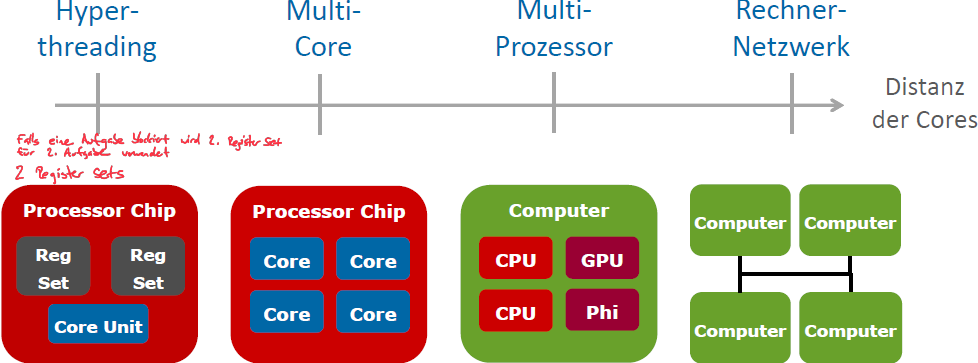
\includegraphics[width=\linewidth]{img/stufen.png}
\textbf{Parallelität:} Aufteilung in Teilabläufe, laufen gleichzeitig auf mehreren Prozessoren.
\textbf{Nebenläufigkeit:} Gleichzeitig oder verzahnt ausführbare Abläufe, greifen au gemeinsame Ressourcen zu.
\textbf{Prozess:} Parallel laufende Programm-Instanz im System. Eigener Adressraum.
\textbf{Thread:} Parallele Ablaufsequenz innerhalb eines Programms. Teilen gleichen Adressraum.

\subsection{Thread-Implementationen}
\textbf{User-Level Threads:} Im Prozess implementiert.
Keine echte Parallelität durch mehrere Prozessoren.
\textbf{Kernel-Level Threads:} Im Kernel implementiert (Multi-Core Ausnutzung).
Kontextwechsel vom Prozess per SW-Interrupt.
\textbf{Thread Scheduling:} Processor Sharing - \#Threads \textgreater \#Prozessoren.

\subsection{Prozessor Multiplexing}
\textbf{Verzahnte Ausführung:} Instruktionen von mehreren Threads in Teilsequenzen. Illusion der Parallelität.
\textbf{Kontextwechsel:} \textit{Synchron} (Freiwillige abgabe), Thread wechselt zu wait. \textit{Asynchron:} (gezwungene Abgabe) Begrenzte Laufzeit für Threads.

\subsection{Multi-Tasking:}
\textbf{Kooperativ:} Threads initiieren Kontextwechsel synchron (freiwillig). Scheduler kann Thread nicht unterbrechen.
\textbf{Preemtiv:} Scheduler kann Thread mit Timer-Interrupt asynchron unterbrechen (Time-Sliced-Scheduling)(\textit{Standart heute}).
\textbf{Thread Zustände:} Ready, Waiting, Running.

\subsection{Multi-Thread Programmierung}
\subsubsection{JVM Thread Modell}
Java ist ein Single Process System. 
JVM ist ein Prozess im Bsys.
\textbf{Main-Thread} wird beim Aufstarten der JVM anhand \textit{main()} Methode erzeugt.
JVM läuft, solange Threads laufen (Ausnahme Daemon Threads).
\begin{lstlisting}
var myThread = new Thread(() -> { /* ... */ });
myThread.start();
\end{lstlisting}
Thread wird erst bei \textit{start()} erzeugt. Führt \textit{run()}-Methode des Runnable Interface aus.
Thread endet beim Verlassen von \textit{run()}.\\
\textbf{Nicht-Determinismus:} Threads laufen ohne Vorkehrungen beliebig verzahnt oder parallel.
\subsubsection{Explizite Runnable-Implementation:}
\begin{lstlisting}
class SimpleLogic implements Runnable {
    @Override
    public void run() { /* ... */ }
}
var myThread = new Thread(new SimpleLogic()).start();
\end{lstlisting}

\subsubsection{Sub-Klasse von Thread}
\begin{lstlisting}
class SimpleThread extends Thread {
    @Override 
    public void run() { /* ... */ }
}
var myThread = new SimpleThread().start();
\end{lstlisting}

\subsubsection{Thread Join}
Warten auf Beendigung eines Threads. \textit{t2.join()} blockiert, solange t2 läuft.

\subsubsection{Thread Passivierung}
\textbf{Thraed.sleep(ms):} Laufender Thread geht in Wartezustand, dann ready.
\textbf{Thread.yield():} Gibt Prozesor frei, direkt ready.
        
\section{Monitor Synchronisation}
\subsection{Java Synchronized Methoden}
\begin{lstlisting}
synchronized void f() { /* ... */ } // Object Lock
static synchronized void g() { /* ... */ } // Class Lock
\end{lstlisting}

\subsection{Monitor}
Objekt mit internem gegenseitigem Ausschluss. Nur 1 Thread operiert im Monitor. Alle äusseren Methoden synchronized.
\textbf{Wait \& Signal Mechanismus:} Threads können im Monitor auf Bedingung warten und wartende aufwecken (signal).

\begin{lstlisting}
public synchronized void withdraw(int a) {
    while (amout > balance) { wait(); }
    balance -= a;
}
public synchronized void deposit(int a) {
    balance+= amount; notifyAll();
}
\end{lstlisting}
\textbf{notify():} Bei Uniform Waiters \& One-In-One-Out Bedingungen.
\textbf{notifyAll():} Bei mehreren Bedingungen / One-In-Multiple-Out. 
\textbf{Pauschales wait \& signal:} Wartende müssen selber schauen, ob sie ein Signal interessiert.
\textbf{Signal and Continue:} Signalisierender Thread behält Monitor nach notify. Aufgeweckter Thread muss um Monitor-Eintritt kämpfen.
        \section{Spezifische Synchronisationsprimitiven}
\subsection{Arten}
\textbf{Faire Semaphoren:} \textit{new Semaphore(N, true)}, FIFO Warteschlange, langsamer.

\begin{lstlisting}
private Semaphore upperL = new Semaphore(CAP, true);
private Semaphore lowerL = new Semaphore(0, true);
public void put(T item) throws InterruptedException {
    upperL.acquire();
    synchronized (queue) { queue.add(item); }
    lowerL.release();
}
public T get() throws InterruptedException {
    T item; lowerL.aquire();
    synchronized (queue) { item = queue.remove(); }
    upperL.release(); return item;
}
\end{lstlisting}
\textbf{Multi-Acquire/Release:} \textit{acquire(N)}.

\subsection{Lock \& Condition}
Monitor mit mehreren Wartelisten für verschiedene Bedingungen.
\textbf{Lock-Objekt:} Sperre für Eintritt in Monitor.
\textbf{Condition-Objekt:} Wait \& Signal für bestimmte Bedingung.

\begin{lstlisting}
private Lock monitor = new ReentrantLock(true); // fair
private Condition nonFull = monitor.newCondition();
private Condition nonEmpty = monitor.newCondition();
public void put(T item) throws InterruptedException {
    monitor.lock();
    try {
        while(queue.size() == Capacity) { nonFull.await(); }
        queue.add(item);
        nonEmpty.signal();
    } finally { monitor.unlock(); }
}
public T get() throws InterruptedException {
    monitor.lock();
    try {
        while(queue.size() == 0) { nonEmpty.await(); }
        T item = queue.remove();
        nonFull.signal();
        return item;
    } finally { monitor.unlock(); }
}
\end{lstlisting}

\subsection{Read-Write Locks}
Gegenseitiger Ausschluss ist unnötig streng für lesende Abschnitte.
Erlaube parallele Lese-Zugriffe.

\begin{lstlisting}
private Collection<String> names = new HashSet<>();
private ReadWriteLock rwLock = new ReentrantReadWriteLock();
public boolean exists(String pattern) { // Read-only accesses
    rwLock.readLock().lock();
    try {
        return names.steram().anyMatch(n -> n.matches(pattern));
    } finally { rwLock.readLock().unlock(); }
}
public void insert(String name) { // Write / Read accesses
    rwLock.writeLock().lock();
    try {
        names.add(name);
    } finally { rwLock.writeLock().unlock(); }
}
\end{lstlisting}

\subsection{Count Down Latch}
Synchronisationsprimitive mit Count Down Zähler.
Threads können warten, bis Zähler <= 0 wird.
\textbf{await():} warten bis Count Down 0 ist.
\textbf{countDown():} Zähler - 1.

\begin{lstlisting}
var ready = new CountDownLatch(N); // Warte auf N cars
var start = new CountDownLatch(1); // Einer gibt signal
// N Cars:
ready.countDown(); start.await();
// RaceControl:
ready.await(); start.countDown();
\end{lstlisting}

\subsection{Cyclic Barrier}
Treffpunkt für fixe Anzahl Threads. Anzahl treffender Threads muss vorgegeben sein.
Ist wiederverwendbar (mehrere Runden).

\begin{lstlisting}
var start = new CyclicBarrier(N); // Treffende Autos
// N Cars:
start.await(); // braucht kein Race Control mehr

var gameRound = new CyclicBarrier(N);
// N Players:
while(true) {
    gameRound.await(); // play concurrently with others
}

// Mit Austausch
Exchanger.exchange(something);
// Blockiert bis anderer Thread auch exchange() aufruft.
\end{lstlisting}
        \section{Gefahren der Nebenläufigkeit}
Neue Arten von Programmierfehler, die es bei single-Threading nicht gibt. 
Können sporadisch oder selten auftreten.
Sehr schwierig durch Tests zu finden.

\subsection{Race Condition}
Mehrere Threads greifen auf gemeinsame Ressourcen ohne genügend synchronisation zu.
Mögliche falsche Resultate oder falsches Verhalten.
Ursache oft ein Data Race, nicht immer.

\subsubsection{Data Race}
Unsynchronisierter Zugriff auf gleichen Speicher.
Selbe Variable oder Array Element (min. 1 schreibender Zugriff).

\subsubsection{Race Condition ohne Data Race}
Critical Sections nicht geschützt. 
Data Races mit Synchronisation eliminiert, aber nicht genügend grosse synchronisierte Blöcke.
\begin{lstlisting}
synchronized int getBalance() { return balance; }
synchronized void setBalance(int x) { balance = x; }
// Mehrere Threads, Kein Atomares Inc - Lost Update moeglich 
accout.setBalance(account.getBalance() + 100);
\end{lstlisting}

\subsubsection{Kombinationen}
\textbf{Alles Synchronisieren?} Hilft nichts. Race Condition trotzdem möglich. Weitere Nebenläufigkeitsfehler.
Synchronisationskosten sind relativ teuer.

\subsection{Synchronisation: Verzichtbare Fälle}
\textbf{Immutability (Unveränderlicheit):} Objekte mit nur lesendem Zugriff.
\textbf{Confinement (Einsperrung):} Objekt gehört nur einem Thread zu einer Zeit.

\subsubsection{Immutable Objects}
Instanzvariablen alle \textit{final}. Primitive Datentypen. Referenzen wiederum auf Immutable Objekte.
Methoden mit nur lesendem Zugriff. Konstruktor initialisiert Instanzvariablen.
Nach Konstruktor kann Objekt ohne Synchronisation von Threads verwendet werden.

\subsubsection{Confinement}
Struktur garantiert, dass auf ein Objekt nur durch einen Thread zur gleichen Zeit zugegriffen wird.
\textbf{Thread Confinement:} Objekt gehört nur einem Thread und wird nur von demjenigen verwendet.
\textbf{Object Confinement:} Objekt in anderem bereits synchronisierten Objekt eingekapselt.\\ 
\textbf{Kapselungsbrüche:} 1. Inneres Objekt ist aussen zugreifbar. 2. Rückgabe einer Referenz auf inneres Objekt.
3. Holder installiert selber Referenz ausserhalb. 4. Inneres Objekt gibt selber \textit{this} raus.


\subsection{Thread Safety}
Klassen / Methoden, die intern synchronisiert sind. Keine Race Conditions innerhalb dieses Codes.
Kritischer Abschnitt nur pro Methode erfüllt.
\textbf{Aber:} Kein kritischer Abschnitt über mehrere Methodenaufrufe. 
Andere Nebenläufigkeitsfehler möglich.

\subsubsection{Java Collections - Thread Safety}
Alte Java 1.0 Collections (Vector, Stack, Hashtable): \textbf{JA}. 
Moderne Collections (HashSet, TreeSet, ArrayList, etc.): \textbf{NEIN}.
Concurrent Collections (ConcurrentHashMap, etc.): \textbf{JA}.

\subsection{Verstecktes Multi-Threading}
\textbf{Finalizers:} Laufen über separaten Finalizer-Thread.
\textbf{Timers:} Handler durch separaten Thread ausgeführt (ausser GUI).
\textbf{Externe Libraries \& Frameworks:} z.B. Abarbeitung von Web-Service Aufrufen.

\subsection{Deadlock}
Beide Threads sperren sich gegenseitig aus:
\begin{lstlisting}
syncrhonized(listA) { // Thread 1
    syncrhonized(listB) {
        listB.addAll(listA);
    }
}
synchronized(listB) { // Thread 2
    synchronized(listA) {
        listA.addAll(listB);
    }
}
\end{lstlisting}

\subsubsection{Spezialfall: Livelocks}
Threads haben sich gegenseitig permanent blockiert. Führen aber noch Warteinstruktionen aus.
Verbrauchen CPU während Deadlock.
\begin{lstlisting}
// Thread 1
b = false; while (!a) { } b = true;
// Thread 2
a = false; while (!b) { } a = true;
\end{lstlisting}

\subsubsection{Deadlock Erkennung}
\textit{Deadlock = Zyklus im Betriebsmittelgraph}\\ 
\textbf{Deadlock Voraussetzungen:} Geschachtelte Locks, Zyklische Warteabhänigkeiten

\subsubsection{Deadlock Vermeidung}
\textbf{Lineare Sperrordnung} der Ressourcen einführen. 
Nur geschachtelt in aufsteigender Reihenfolge sperren. 
Eliminiert zyklische Warteabhänigkeiten.\\ 
\textbf{Grobgranulare Locks} wählen.
Wenn lineare Sperrordnung nicht möglich/sinvoll ist.
Sperre gesamte Bank bei Kontenzugriff.
Eliminiert Schachtelung von Locks.

\subsection{Starvation}
Ein Thread kriegt nie die Chance, auf eine Ressource zuzugreifen, obwohl sie immer wieder frei wird.
Andere Threads überholen andauernd. Liveness/Fairness Problem.
\begin{lstlisting}
do { // Starvation moeglich 
    success = account.widthdraw(100);
} while (!success);
\end{lstlisting}

\subsubsection{Vermeidung}
Faire Synchronisationskonstrukte (bei Semaphore, Lock \& Condition, ReadwriteLock möglich).
Java Monitor hat ein Fairness Problem (Starvation anfällig).

\subsection{Parallelität Korrektheitskriterien}
\textbf{Safety:} Keine Race Conditions, Keine Deadlocks.
\textbf{Liveness:} Keine Starvation.
        \section{Thread Pool}
\textbf{Tasks:} Implementieren potentiell parallele Arbeitspakete. Werden in Warteschlange eingereiht.
\textbf{Thread Pool:} Beschränkte Anzahl von Worker-Threads.
Holen Tasks aus der Warteschlange und führen sie aus.

\subsection{Vorteile}
\textbf{Beschränkte Anzahl von Threads:} Viele Threads verlangsamen das System oder überschreiten Speicherlimit. 
\textbf{Recycling der Threads:} Spare Thread-Erzeugung und Freigabe.
\textbf{Höhere Abstraktion:} Trenne Task-Beschreibung von Task-Ausführung.
\textbf{Anzahl Threads pro System konfigurierbar:} \#Worker Threads = \#Prozessoren + \#I/O-Aufrufe 

\subsection{Einschränkung}
Tasks dürfen nicht aufeinander Warten, sonst Deadlock.
\textbf{Run to Completion:} Task muss zu Ende laufen, bevor Worker Thread anderen Task ausführen kann.
\textbf{Ausnahme:} geschachtelte Tasks.

\subsection{Java Fork-Join-Pool}
\begin{lstlisting}
var threadPool = new ForkJoinPool();
Future<Integer> future = threadPool.submit(() -> {  });
Int result = future.get(); // Blockiert bis Task beendet
\end{lstlisting}

\subsubsection{Future Konzept}
Repräsentiert ein zukünftiges Resultat.
Proxy auf Resultat, das evtl. noch nicht bekannt ist. 
Muss Ende der Berechnung abwarten, bevor Resultat zurückgegeben wird.

\subsubsection{Rekursive Task Erstellung}
\begin{lstlisting}
class CountTask extends RecursiveTask<Integer> {
    // Constructor
    @Override
    protected Integer compute() {
        // no / single element => return result
        // Calculate lower, middle, upper
        var left = new CountTask(lower, middle);
        var right = new CountTask(middle, upper);
        left.fork(); right.fork();
        return right.join() + left.join(); } }
// Ausfuehrung 
var threadPool = new ForkJoinPool();
int res = threadPool.invoke(new CountTask(2, N)); // blockiert
\end{lstlisting}

\subsubsection{Keine Über-Parallelisierung}
Tuning mit Schwellwert durch Programmierer.
Verhältnis zwischen Arbeitspaketgrösse und Anzahl Tasks optimieren.

\subsubsection{Fork Join Pool Internals}
\textbf{Automatischer Parallelitätsgrad:} Default: \#Worker Threads = \#Prozessoren
Dynamisches Hinzufügen / Wegnehmen von Threads
\textbf{Common Pool:} Verhindert Engpässe durch zu viele Thread Pools.


\subsection{Asynchrone Programmierung}
\textbf{Unnötige Synchronität:} Langlaufende Rechnungen, I/O Aufrufe.\\ 
\textbf{Asynchroner Aufruf:} Aufrufer soll während der Operation weitermachen.

\begin{lstlisting}
// Klassisch
Future<long> future = threadPool.submit(() -> { });
    // other work 
process(future.get());
// Modern
CompletableFuture<long> future = 
                    CompletableFuture.supplyAsync(() -> { });
    // other work 
process(future.get());
\end{lstlisting}

\subsubsection{Ende des async Aufrufs}
\textbf{Caller-zentrisch (Pull):} Caller warted auf Task-Ende und holt sich Resultat, Future abfragen.
\textbf{Callee-zentrisch (Push):} Async Operation informiert direkt über Resultat. Completion Callback.

\subsubsection{Continuation}
Folgeaufgabe an asynchrone Aufgabe anhängen.
\begin{lstlisting}
// thenApply() fuer Continuation mit Rueckgabe
future.thenAccept(res -> System.out.println(res));
\end{lstlisting}
\textbf{Ausführung:} durch beliebigen Thread, durch Initiator, wenn Future bereits Resultat hat.
\textbf{Asynchrone Continuations:} \textit{thenAcceptAsync()} bzw. \textit{thenApplyAsync()}.

\subsubsection{Multi-Continuation}
\begin{lstlisting}
CompletableFuture.allOf(f1, f2).thenAcceptAsync(() -> { }));
CompletableFuture.any(f1, f2).thenAcceptAsync(() -> { }));
\end{lstlisting}

\subsubsection{Fire and Forget}
Task starten, ohne das Ende abzuwarten. Submitter ruft kein \textit{get()} oder \textit{join()} auf.
\begin{lstlisting}
CompletableFuture.runAsync(() -> { });
\end{lstlisting}
\textbf{Daemon Workers:} Workers Threads in Fork-Join-Pools sind Daemon.
Anwendung kann vor Task-Ende stoppen.\\ 
\textbf{Ingorierte Exceptions:} Exceptions in Fire \& Forget Task werden ignoriert.

        \section{Task Parallel Library}
\subsection{.NET Threads}
\textbf{Keine Vererbung:} Delegate bei Konstruktor.
\textbf{Exception in Thread:} Abbruch des Programs.
\begin{lstlisting}[language=csh]
var myThread = new Thread(() => { /* ... */ });
myThread.start(); /* ... */ myThread.join();
\end{lstlisting}
C\# Lambda kann umgebende Variablen zugreifen (auch scrheibend).

\subsection{Monitor in .NET}
FIFO Warteschlange, Pulse informiert längst Wartenden. \textit{Wait()} in Schlaufe.
\textit{PulseAll()} bi mehreren Bedingungen oder Erfüllungen mehrerer Threads.
Synchronisation mit HilfsObj als Best Practice.
\begin{lstlisting}[language=csh]
private object syncObject = new(); // Monitor auf HilfsObj
public void Widthdraw(decimal amount) {
    lock (syncObject) {
        while(amout > balance) { Monitor.Wait(syncObject); }
        balance -= amount; } }
public void Deposit(decimal amount) {
    lock (syncObject) {
        balance += amount;
        Monitor.PulseAll(syncObject);  } }
\end{lstlisting}

\subsection{.NET Synchronisationsprimitiven}
\textbf{Fehlen:} kein Fairnessflag, kein Lock \& Condition.
\textbf{Zusätzlich:} ReadwriteLockSlim für Upgradeable Read/Write. Semaphoren auch auf OS-Stufe nutzbar.
Mutex (binärer Semaphor).
\textbf{Collections nicht Thread-safe:} Ausser \textit{System.Collections.Concurrent}

\subsection{.NET Task Parallel Library (TPL)}
Work Stealing Thread Pool. 
\textbf{Verschiedene Abstraktionsstufen:} Task Parallelization: Explizite Tasks starten und warten.
Data Parallelization: Parallele Statements und Queries.
Asynchrone Programmierung: mit Continuation Style.

\subsubsection{Thread Injection}
TPL fügt zur Laufzeit neue Worker Threads hinzu.
\textbf{Hill Climbing Algorithmus:} Misst Durchsatz \& variiert Anzahl Worker Threads.
\textbf{Kein Deadlock} bei Task Abhängigkeiten, aber ineffizient, nicht dafür gemacht.

\subsection{Task Parallelisierung}
\begin{lstlisting}[language=csh]
Task task = Task.Run(() => { }); /* ... */ task.Wait();
// Task mit Rueckgabe 
Task<int> task = Task.Run(() => { return 0; });
Console.Write(task.Result); // Blockiert 
// Geschachtelte Tasks
Task.Run(() => {
    var left = Task.Run(() => { }); 
    var right = Task.Run(() => { });
    int res = left.Result + right.Result; });
\end{lstlisting}

\subsubsection{Parallele Statements}
Menge an Statements potentiell parallel ausführen. Als Task starten. Barriere der Tasks am Ende.
\begin{lstlisting}[language=csh]
Parallel.Invoke(
    () => MergeSort(l, m); () => MergeSort(m,l);
);
\end{lstlisting}

\subsubsection{Parallele Loop}
Schlaufen-Bodies potentiell parallel ausführen.
Gruppierung der Bodies in Tasks.
Berriere dieser Tasks am Ende.
\begin{lstlisting}[language=csh]
Parallel.ForEach(list, file => Convert(file));
Parallel.For(0, array.Length, i => Calc(array[i]));
\end{lstlisting}

\subsubsection{Parallele Loop Partitionierung}
Schlaufe mit vielen sehr kurzen Bodies ist ineffizient.
TPL gruppiert automatisch mehrere Bodies zu Task.
Aufteilung gemäss verfügbaren Worker Threads.\\
\textbf{Explizite Partitionierung:} Vorteil: Weniger Body-Delegates, Nachteil: Künstliche Unterschleife.
\begin{lstlisting}[language=csh]
Parallel.ForEach(Partitioner.Create(0, array.Length), 
    (range, _) => {
        for (int i = range.Item1; i < range.Item2; i++) {
            Calc(array[i]);
        } })
\end{lstlisting}

\subsection{Asynchrone Programmierung mit TPL}
\subsubsection{Task Continuation}
\begin{lstlisting}[language=csh]
task1.ContinueWith(task2).ContinueWith(task3);
// Multi-Continuation
Task.WhenAll(task1, task2).ContinueWith(continuation);
Task.WhenAny(task1, task2).ContinueWith(continuation);
\end{lstlisting}


        \section{GUI and Threading}
GUI Frameworks erlauben nur Single-Threading. \\ 
\textbf{UI Thread:} Loop zur Ausführung der Ereignisse aus einer Queue.
\subsection{UI Thread Confinement}
Wiso basieren GUI-Frameworks auf Single-Thread Modell?\\
\textbf{Synchronisationskosten:} Locking in allen Komponenten und Methoden relativ teuer.
\textbf{Deadlock-Risiko:} Bei zyklischen geschachtelten Aufrufen (z.B. MVC).

\subsection{Swing: Dispatching an UI Thread}
Komponentenzugriffe an UI Thread delegieren.
\begin{lstlisting}
// Benutzung der Klasse SwingUtilities
static void invokeLater(Runnable doRun); // Async
static void invokeAndWait(Runnable doRun); // Synchron 
// Example unordered, parallel link check
button.addActionListener(e -> {
    var url = input.getText();
    CompletableFuture.runAsync(() -> {
        var html = webClient.download(url); // blocking
        for(var link : webClient.extractLinks(html)) {
            CompletableFuture.runAsync(() -> {
                if(!webClient.isAccessible(link)) {
                    SwingUtilities.invokeLater(() -> 
                        output.addElement(link + " is broken"));
                }
            })
        }
    });
});

// Example (same order of downloads) - Recursive
void download(List<URL> links, OutputStream output) {
    if(links.isEmpty()) {
        statusLabel.setText("All done!");
    }
    var url = links.get(0);
    statusLabel.setText("Downloading" + url);
    if(cancelBox.isSelected()) {
        statusLabel.setText("cancelled!");
        return;
    }
    CompletableFuture.runAsync(() -> {
        url.openStream().transferTo(output);
        var remaining = links.subList(1, links.size());
        SwingUtilities.invokeLater(() -> download(remaining, output));
    });
}
\end{lstlisting}

\subsection{.NET UI Threading Modell}
Gleiches Prinzip wie Java.
\textbf{UI Thread:} Aufrufer von \textit{Application.Run()}.\\ 
\textbf{UI Event Dispatching:}
WPF: \textit{control.Dispatcher.InvokeAsync(action)}\\ 
WinForm: \textit{control.BeginInvoke(delegate)}

\subsubsection{Async / Await}
Async Methode läuft teilweise synchron, teilweise asynchron.
Aufrufer führt Methode solange synchron aus bis ein \textit{await} anliegt.
Compiler zerlegt Methode in Abschnitte. Abschnitt nach Await läuft später nach Task-Ende (Continuation).
Methode läuft synchron bis \textit{await}, springt dann zurück zum Aufrufer.\\ 
\textbf{Verschiedene Ausführungen:} Fall 1: Aufrufer ist normaler Thread, Abschnitt wird durch TPL Worker-Thread ausgeführt.
Fall 2: Aufrufer ist UI-Thread, Abschnitt wird als Event vom UI-Thread ausgeführt.
\begin{lstlisting}[language=csh]
public async Task<int> LongOperationAsync() { }
Task<int> task = LongOperationAsync(); /* ... */
int res = await task; // Warte auf Beendigung
\end{lstlisting}
\textbf{Async Rückgabetypen:}
\textit{void}: fire-and-forget.
\textit{Task}: Kein Rückgabetyp erlaubt warten.
\textit{Task\textless T\textgreater} Rückgabetyp T.
\begin{lstlisting}[language=csh]
async Task<string> ConcatAsync(string url1, string url2) {
    HttpClient client = new HttpClient();
    Task<string> d1 = client.GetStringAsync(url1);
    Task<string> d2 = client.GetStringAsync(url2);
    string site1 = await d1; string site2 = await d2;
    return site1 + site2;
}
\end{lstlisting}
        \section{Memory Models}
\textbf{Lock-Freie Programmierung:} Korrekte nebenläufige Interaktionen ohne Locks.
Garantien des Speichermodels nutzen.
\subsection{Ursachen für Probleme}
\textbf{Weak Consistency:} Speicherzugriffe werden in verschiedenen Reihenfolgen aus verschiedenen Threads gesehen.
Ausnahme: Synchronisationen/Speicherbarrieren
\textbf{Optimierungen:} Compiler, Laufzeitsystem und CPUs, Instruktionen werden umgeordnet/wegoptimiert.

\subsection{Java Memory Model}
\subsubsection{Atomicity}
Einzelnes Lesen / Schreiben ist atomar für: Primitive Datentypen, Obj-Referenzen, long und double nur mit \textit{volatile} Keyword.\\ 
\textbf{Unteilbarkeit $\neq$ Sichtbarkeit:} Nach Write sieht anderer Thread vlt. noch alten Wert.

\subsubsection{Visibility}
\textbf{Garantierte Sichtbarkeit zwischen Threads:}
Locks Release \& Acquire, Volatile Variable, Thread/Task-Start und Join, Initialisierung von final Variablen.

\subsubsection{Ordering}
\textbf{Program Order:} 'as-if-serial', Sequentielles Verhalten jedes Threads bleibt erhalten. (Andere Threads dürfen es anders sehen)
\textbf{Synchronization Order (Total Order):} Synchronizationsbefehle werden zueinander nie umgeordnet.
\textbf{Happens-Before Relation (Partial Order):} Alles andere kann umgeordnet werden, ausser es gibt garantierte Sichtbarkeit unter den Threads.

\subsection{Java Synchronization Order}
\begin{lstlisting}
// Keine Umordnung in Java, weil alles volatile
volatile boolean a = false, b = false;
a = true; while(!b) { } // Thread 1 
b = true; while(!a) { } // Thread 2 
// Nicht korrekt, da nicht atomar 
private volatile boolean locked = false;
public void aqcuire() {
    while(locked) { }
    locked = true;
}
// Spin-Lock mit atomarer Operation
private AtomicBoolean locked = new AtomicBoolean(false);
public void acquire() {
    while (locked.getAndSet(true)) { }
}
public void release() { locked.set(false); }
// Atomares Compare and Set, setzt Update falls Wert gleich expect
boolean compareAndSet(boolean expect, boolean upadte);
// Optimistische Synchronization
do {
    oldValue = var.get(); newValue = calcChange(oldValue);
} while (!var.compareAndSet(oldValue, newValue));
\end{lstlisting}

\subsection{.NET Memory Model}
\textbf{Unterschied zu Java:} Atomicity: long/double auch ohne volatile atomar.
Visibility: Nicht definiert, implizit durch Ordering.
Ordering: nur Half und Full Fences.\\ 
\textbf{Atomare Instruktionen:} \textit{Interlocked} Klasse

\subsubsection{Volatile Half Fences}
\textbf{Volatile Write:} Vorangehende Zugriffe bleiben davor. (Release Semantik)
\textbf{Volatile Read:} Nachfolgende Zugriffe bleiben danach. (Acquire Semantik)

\subsubsection{Full Fence: Memory Berrier}
\begin{lstlisting}[language=csh]
Thread.MemoryBarrier(); // Verbietet Umordnung in beide Richtungen
\end{lstlisting}
        \section{Actor Model}
\textbf{Async:} nicht Blockierend.\\
Substantiell anderes Programmierkonzept.
\textbf{Aktive Objekte:} haben nebenläufiges Innenleben.
\textbf{Kommunikation:} Objekte senden und empfangen Nachrichten.
\textbf{Kein Shared Memory:} Nur Austausch von Nachrichten.

\subsection{Vorteile: Actor, CSP} 
\textbf{Inhäerente Nebenläufigkeit:} Alle Obj (Actors) laufen nebenläufig.
Maschine kann Grad an Nebenläufigkeit ausnutzen.
\textbf{Keine Race Conditions:} Kein Shared Memory. Nachrichtenaustausch synchronisiert implizit.
\textbf{Gute Verteilbarkeit:} Kein Shared Memory. 
Nachrichtenaustausch für Netz prädestiniert.

\subsection{Akka}
Actor Model für JVM. Actors haben privaten Zustand, kann aber auf JVM nicht enforced werden.
Eine Mailbox pro Actor: Ein Buffer für alle ankommenden Nachrichten. Asynchones Senden.\\ 
\textbf{Empfangsverhalten:} Reaktion auf ankommende Nachricht. Behandlungsmethode wird ausgeführt.
Effekte per Behandlung (Ändere Zustand, Sende Nachrichten, Erzeuge neue Actors).
Intern sequentiell, nur eine Nachricht auf einmal behandelbar.
\begin{lstlisting}
public class Printer extends UntypedActor {
    public void onReceive(final Object message) {
        if(message instanceof Integer) { } } }
// Erzeugen und Senden
ActorSystem system = ActorSystem.create("System");
ActorRef p = system.actorOf(Props.create(Printer.class));
for(int i = 0; i < 100; i++) {
    printer.tell(i, ActorRef.noSender()); // simple async
}
System.shutdown();
\end{lstlisting}

\textbf{Anwendung:}
Alternative zu Threads, Transaction-Processing, 
Backend für Service, Kommunikations-Hub.\\ 
\textbf{Actor Hierarchies:}
Passend zu URL Adressierungsschema. Erzeuger ist Parent. 
\textit{ActorSelection} selektiert Teilbaum, broadcast möglich.

        \section{GPU Parallelisierung}
512, 1024, 3584, 5760 Cores. 
Sehr spezifische langsamere Prozessoren.
\subsection{GPU Aufbau}
\textbf{SP (Streaming Processor):} 8-192 SPs pro SM 
\textbf{SM (Streaming Multiprocessor):} z.B. 1-30 SM
\textbf{SIMD:} SM ist prinzipiell SIMD (Single Instruction Multiple Data), Vektorparallelität
Alle Cores führen gleiche Instruktion aus, Einzelne können sie auch nicht ausführen.

\subsection{GPU vs. CPU}
\textbf{GPU:} hohe Datenparallelität, wenig Verzweigungen, Kein beliebiges Warten, Kleine Caches pro Core. Ziel: Hoher Gesamtdurchsatz
\textbf{CPU:} Gegenteil, Ziel: Niedrige Latenz pro Thread

\subsection{NUMA Modell}
\textbf{Non-Uniform-Memory-Access:} Kein gemeinsamer Hauptspeicher zwischen GPU und CPU.
Explizites Übertragen.

\subsection{CUDA - Computer Unified Device Architecture}
\textbf{CUDA Blocks:} Threads sind in Blöcke gruppiert.
Blöcke sind im gleichen SM. Threads können innerhalb Block interagieren.
\textbf{Ausführungsmodell:}
Thread: virt. Skalarprozessor. 
Block: virt. Multiprozessor.
Blöcke müssen unabhängig sein. Run To Completion.
Beliebige Ausführungsreihenfolge.
Grad der Parallelität durch GPU bestimmt. 
Automatische Skalierung.
\textbf{Ablauf:} 1. Auf GPU allozieren \textit{cudaMalloc}, 
2. Daten au GPU transferieren \textit{cudaMemcpy},
3. Kernel ausführen,
4. Rücktransfer, 
5. Auf GPU deallozieren

\subsubsection{Datenaufteilung}
\textbf{threadIdx.x:} ThreadId im Block.
\textbf{blockIdx.x:} Nummer des Blocks.
\textbf{blockDim.x:} Blockgrösse.
Programmierende modellieren Datenaufteilung selber.

\subsubsection{Boundary Check}
Falls Mehr Threads als zu bearbeitende Daten.
Threads mit $i \geq N$ dürfen nicht auf Daten zugreifen.

\subsubsection{Unified Memory}
Automatischer Transfer CPU - GPU.

        \subsection{Speicherstufen}
\textbf{Shared Memory:} Per SM.
Schnell ca 4 Zyklen.
Nur zwischen Threads innerhalb Block sichtbar.
Paar KB.
\textit{\_\_shared\_\_ float x;}
\textbf{Global Memory:}
Main Memory in GPU.
Langsam, ca. 400-600 Zyklen.
Allen Threads sichtbar.
Mehrere GB.
\textit{cudaMalloc()}

\subsection{Block Barriere}
\begin{lstlisting}
__syncThreads();
\end{lstlisting}
In if/else nur falls für alle Threads eines Blocks.

\subsection{Warp}
Block wird intern in Warps zerlegt (je 32 Threads).
\textbf{Ausführung:} SIMD.
SM kann alle Warps eines Blocks beherbergen. Nur wenige laufen echt parallel (1 bis 24).

\subsection{Divergenz}
Unterschiedliche Verzweigungen im selben Warp.
\textit{if/switch/while/do/for}.
SM führt Intruktionen der einen Verzweigung durch, dann Instruktionen einer anderen Verzweigung.
\textbf{Performance Problem}
Schlechter Fall: Divergenz innerhlab derselben Warp.
Guter Fall: Gleiche Verzweigung im Warp.

\subsection{Memory Coalescing}
Zugriffsmuster für Performance optimieren.
\textbf{Burst:}  Falls Threads auf 32-Byte-Bereiche zugreifen.
Sonst teure Einzel-Zugriffe. (je 400 Zyklen pro Global Memory)\\ 
\textbf{Tiles einlesen}, \textbf{Multi-Dim} Spalte auf x-Achse

\subsection{Shared Memory Optimization}
Falls Threads auf mehrere Elemente zugreifen, im SM Cachen.

\subsection{Example}
\subsubsection{1-Dimensional}
\begin{lstlisting}
__global__ void pairwise_sum(int* array, int length) {
    int i = blockIdx.x * blockDim.x + threadIdx.x;
    int offset = 2 * i;
    if(offset + 1 < length) {
        array[offset] += array[offset + 1];
        array[offset + 1] = 0;
    }
}
// Aufruf
int blockSize = 1024;
int gridSize = (len / 2 + blockSize - 1) / blockSize;
pairwise_sum<<<gridSize, blockSize>>>(d_a, len);
\end{lstlisting}

\subsubsection{2-Dimensional}
\begin{lstlisting}
__global__ void transpose(int* matrix, int rows, int cols, int* result) {
    int row = blockIdx.x * blockDim.x + threadIdx.x;
    int col = blockIdx.y * blockDim.y + threadIdx.y;
    if(row < rows && col < cols) {
        result[col * rows + row] = matrix[row * cols + col];
    }
}
// Aufruf
dim3 blockSize(32,32);
dim3 gridSize((N + 31) / 32, (M + 31) / 32);
transpose<<<gridSize, blockSize>>>(matrix, N, M, result);
\end{lstlisting}
        \section{Cluster Parallelisierung}
\textbf{Motivation:} möglichst hohe Beschleunigung. Viele CPU Cores statt nur viele GPU Cores.
\textbf{Computer Cluster:} Verbund leistungsfähiger Rechenknoten.
Meist gleichartig und fest verbunden an einem Standort. Sehr schnelles Interconnect.
\textbf{HPC Anleitung:} Programcode uploaden, Auf Cluster Kompilieren, HPC-Job lancieren, Job-Ende abwarten, Job-Resultat anschauen.
\textbf{Verteiltes Programmiermodel:} Programm auf mehreren Nodes ausführen. Kein Shared Memory (NUMA) zwischen nodes, nur für Cores im Node (SMP).
\textbf{Message Passing Interface (MPI):} Basiert auf Actor/CSP Prinzip.
\begin{lstlisting}
MPI_Init(&argc, &argv); // MPI Initialisierung 
MPI_Comm_rank(MPI_COMM_WORLD, &rank); // Prozess Identifikation
MPI_Finalize(); // MPI Finalisierung
MPI_Send(&val, 1, MPI_INT, recRank, tag, MPI_COMM_WORLD);
MPI_Recv(&val, 1, MPI_INT, senderRank, tag, MPI_COMM_WORLD, 
                                        MPI_STATUS_IGNORE);
MPI_Barrier(MPI_COMM_WORLD); // Wartet auf alle Prozesse
MPI_Allreduce(&val, &total, 1, MPI_INT, MPI_SUM, 
    MPI_COMM_WORLD); // Aggregation von Teilresultaten
MPI_Reduce(&val, &total, 1, MPI_INT, MPI_SUM, recRank, 
    MPI_COMM_WORLD); // Effizienter, kein Broadcast
\end{lstlisting}
\textbf{SPMD:} Single Program Multiple Data. MPI Programm wird in mehrere Prozesse gestart.
Prozesse können untereinander kommunizieren.
\textbf{Communicator:} Gruppe von MPI-Prozessen. 
Communicator World: Alle Prozesse einer MPI-Programmausführung.
        \section{Concurrency in Python}
\textbf{GIL:} Global Interpreter Lock. 
Nur ein Thread kann Python Byte-Code ausführen.
Kein Speedup für CPU-Bount Operationen möglich. Data Races durch Reordering dennoch möglich, Visibility nicht garantiert.
Kein definiertes Memory Model.
\begin{lstlisting}[language=python]
from threading import Thread
from multiprocessing import Process
if __name__ == '__main__':
    t = Thread( # p = Process
        target=fibonacci,
        args=(10,)
    ).start();
    t.join();
# Shared Memory
res = Value('i', -1, lock=False); // Typ, InitialWert, lock
\end{lstlisting}

\subsection{Pools}
\textbf{Threads:} \textit{concurrent.futures.thread.ThreadPoolExecutor}
\textbf{Prozesse:} \textit{concurrent.futures.process.ProcessPoolExecutor} / \textit{multiprocessing.Pool}
\begin{lstlisting}[language=python]
if __name__ == '__main__':
    with ProcessPoolExecutor() as pool:
        future = pool.submit(fib, 10) # or: map(fib, [1,2,3])
        print(future.res()); # Blockiert bis Task-Ende
\end{lstlisting}

\subsection{Asnychrone Programmierung (asyncio)}
\textbf{Coroutine-Functions:} werden erst beim \textit{await} ausgeführt.
Keine parallele Ausführung. Ausnahme: Coroutine wird als Task verpackt.
\begin{lstlisting}[language=python]
async def sub_routine(n):
    await asyncio.sleep(n);
if __name__ == 'main__':
    asyncio.run(sub_routine(1))
\end{lstlisting}


\section{JavaScript Concurrency}
Grundsätzlich Single-Threaded mit einem Event-Loop.
Kein Schutz vor Race-Condition.
\begin{lstlisting}
function delay(ms) {
    let promise = new Promise((resolve, reject) => {
    setTimeout(() => resolve(), ms); }); }
async function countTo(n) {
    for (let = 1; i <= n; i++) {
        await delay(1000); } }
\end{lstlisting}
\subsection{Web-Worker}
Entsprechen einem Thread im Browser. Datenaustausch primär über Messaging.
Werden mit Quelldatei gestartet. Langlebiger Prozess mit eigenem Event-Loop.
\begin{lstlisting}
onmessage = event => { // Worker definieren
    const n = event.data; const res = fib(n);
    postMessage(res); }
const worker = new Worker('w.js'); // Worker verwenden
worker.onmessage = event => {
    console.log(event.data); }
worker.postMessage(42);
\end{lstlisting}

    \end{multicols*}
\end{document}

























